\documentclass[9pt]{beamer}
% !TeX root = main.tex
% this template mostly comes from Trinkle23897
% his github repo is https://github.com/Trinkle23897/THU-Beamer-Theme
% thanks a lot Trinkle!
% two color theme fdu_red and fdu_blue, choose your preference main document and switch in the menu
% github repo https://github.com/milanmarks/FDU-Beamer-Theme
\usepackage{ctex, hyperref}
\usepackage[T1]{fontenc}
\usepackage{ulem}
\usepackage{bbm}
\usepackage{turnstile}
\usepackage{amsfonts}
\usepackage{subcaption}
\usepackage{mathrsfs}
% other packages
\usepackage{latexsym,amsmath,xcolor,multicol,booktabs,calligra}
\usepackage{graphicx,pstricks,listings,stackengine}
\usepackage[numberedbib]{apacite}
\usepackage{natbib}

\newtheorem{remark}{Remark}



%%%%%%%%% Basic Information %%%%%%%%%%%%%%%%%
\author{Chen Yang author}
\title{12.1.1 Maximum-Variance Formulation of PCA}
\subtitle{Pattern Recognition and Machine Learning, C.M.Bishop}
\institute{School of Data Science, Fudan University}
\date{$8^{th}$ December, $2025$}
\usepackage{Tsinghua_fdured}


% defs
\def\cmd#1{\texttt{\color{red}\footnotesize $\backslash$#1}}
\def\env#1{\texttt{\color{blue}\footnotesize #1}}
\definecolor{deepblue}{rgb}{0,0,0.5}
\definecolor{deepred}{rgb}{0.6,0,0}
\definecolor{deepgreen}{rgb}{0,0.5,0}
\definecolor{halfgray}{gray}{0.55}

\lstset{
    basicstyle=\ttfamily\small,
    keywordstyle=\bfseries\color{deepblue},
    emphstyle=\ttfamily\color{deepred},    % Custom highlighting style
    stringstyle=\color{deepgreen},
    numbers=left,
    numberstyle=\small\color{halfgray},
    rulesepcolor=\color{red!20!green!20!blue!20},
    frame=shadowbox,
}

\def \H{\mathbf{H}}
\def \M{\mathbf{M}}
\def \cA{\mathcal{A}}
\def \cC{\mathcal{C}}
\def \cF{\mathcal{F}}
\def \cG{\mathcal{G}}
\def \cH{\mathcal{H}}
\def \cU{\mathcal{U}}
\def \cV{\mathcal{V}}
\def \cX{\mathcal{X}}
\def \cY{\mathcal{Y}}
\def \cZ{\mathcal{Z}}
\def \mH{\mathcal{H}}
\def \mC{\mathcal{C}}
\def \mU{\mathbb{U}}
\def \mZ{\mathbb{Z}}
\def \mS{\mathbb{S}}
\def \mD{\mathscr{D}}
\def \mA{\mathcal{A}}
\def \EY{E(\overline{Y}_n(\boldsymbol{x}^*))}
\def \bD{\boldsymbol{D}}
\def \bY{\boldsymbol{Y}}
\def \bA{\boldsymbol{A}}
\def \B{\boldsymbol{B}}
\def \a{\boldsymbol{a}}
\def \e{\boldsymbol{e}}
\def \F{\boldsymbol{F}}
\def \w{\boldsymbol{w}}
\def \Z{\boldsymbol{Z}}
\def \W{\boldsymbol{W}}
\def \V{\boldsymbol{V}}
\def \X{\boldsymbol{X}}
\def \bx{\boldsymbol{x}}
\def \f{\boldsymbol{f}}
\def \bC{\boldsymbol{C}}
\def \bc{\boldsymbol{c}}
\def \by{\boldsymbol{y}}
\def \bv{\boldsymbol{v}}
\def \bw{\boldsymbol{w}}
\def \bV{\boldsymbol{V}}
\def \bW{\boldsymbol{W}}
\def \bO{\boldsymbol{O}}
\def \inde{\rotatebox[origin=c]{90}{$\models$}}
\def \RR{\text{RR}}
\def \mP{\mathbb{P}}
\def \P{\mathbf{P}}
\def \Q{\mathbf{Q}}
\def \K{\mathbf{K}}
\def \U{\mathbf{U}}
\def \D{\mathbf{D}}
\def \V{\mathbf{V}}
\def \v{\mathbf{v}}
\def \h{\mathbf{h}}
\def \x{\mathbf{x}}
\def \W{\mathbf{W}}
\def \Y{\mathbf{Y}}
\def \s{\mathbf{s}}
\def \A{\mathbf{A}}
\def \mR{\mathbb{R}}
\def \mE{\mathbb{E}}
\def \mI{\mathbb{I}}
\def \bxi{\boldsymbol{\xi}}
\def \bmu{\boldsymbol{\mu}}
\def \bPhi{\boldsymbol{\Phi}}
\def \bSigma{\boldsymbol{\Sigma}}
\def \bbeta{\boldsymbol{\beta}}
\def \bgamma{\boldsymbol{\gamma}}
\def \bpsi{\boldsymbol{\psi}}
\def \bfeta{\boldsymbol{\eta}}
\def \bPsi{\boldsymbol{\Psi}}
\def \blambda{\boldsymbol{\lambda}}
\def \bLambda{\boldsymbol{\Lambda}}
\def \bTheta{\boldsymbol{\Theta}}
\def \bPi{\boldsymbol{\Pi}}
\def \bOmega{\boldsymbol{\Omega}}
\def \bzeta{\boldsymbol{\zeta}}
\def \btheta{\boldsymbol{\theta}}
\def \bsigma{\boldsymbol{\sigma}}
\def \R{\mathbf{R}}
\def \p{\mathbf{p}}
\def \b{\mathbf{b}}
\def \g{\mathbf{g}}
\def \k{\mathbf{k}}
\def \z{\mathbf{z}}
\def \y{\mathbf{y}}
\def \O{\mathcal{O}}
\def \bZ{\boldsymbol{Z}}

\def \wh{\widehat}
\def \wt{\widetilde}
\def\defeq{\stackrel{\mathrm{def}}{=}}  % for definitions

\def \mN{\mathbb{N}}
\def \mQ{\mathbb{Q}}

\def \cA{\mathcal{A}}
\def \cB{\mathcal{B}}
\def \cC{\mathcal{C}}
\def \cD{\mathcal{D}}
\def \cE{\mathcal{E}}
\def \cF{\mathcal{F}}
\def \cG{\mathcal{G}}
\def \cH{\mathcal{H}}
\def \cK{\mathcal{K}}
\def \cL{\mathcal{L}}
\def \cM{\mathcal{M}}
\def \cN{\mathcal{N}}
\def \cO{\mathcal{O}}
\def \cP{\mathcal{P}}
\def \cQ{\mathcal{Q}}
\def \cR{\mathcal{R}}
\def \cS{\mathcal{S}}
\def \cU{\mathcal{U}}
\def \cW{\mathcal{W}}
\def \cX{\mathcal{X}}
\def \cY{\mathcal{Y}}
\def \scrX{\mathscr{X}}
\def \scrD{\mathscr{D}}
\def \scrC{\mathscr{C}}
\def \cI{\mathcal{I}}
\def \cS{\mathcal{S}}
\def \cT{\mathcal{T}}
\def \scrl{\mathscr{l}}
\def \cZ{\mathcal{Z}}

\def \bcalP{\boldsymbol{\mathcal{P}}}
\def \bpi{\boldsymbol{\pi}}
\def \brho{\boldsymbol{\rho}}
\def \bkappa{\boldsymbol{\kappa}}
\def \bepsilon{\boldsymbol{\epsilon}}
\def \f{\boldsymbol{f}}

\def \E{\mathbb{E}}
\def \zero{\mathbf{0}}
\def \I{\mathbf{I}}
\def \tr{\mbox{Tr}}
\def \cov{\mbox{cov}}

\def \ol{\overline}
\def \one{\mathbf{1}} 
\def \Var{\textup{Var}} 

\graphicspath{{../pic/}}
\begin{document}

\begin{frame}
    \titlepage
    \centering
\end{frame}

\section{Introduction}


\begin{frame}{Motivation}

\textbf{Why do we need PCA?}
\begin{itemize}
  \item Modern data sets often live in a high-dimensional ambient space $\mR^D$ (images, text features, genomic data, \dots).
  \item Directly working in this space is expensive and can hide the essential structure of the data.
  \item Principal Component Analysis (PCA) is a linear dimensionality reduction method that searches for directions along which the data vary the most.
\end{itemize}

\textbf{Focus of this talk}
\begin{itemize}
  \item We follow Section 12.1.1 of \emph{Pattern Recognition and Machine Learning} (Bishop, 2006).
  \item We explain the \emph{maximum-variance formulation} of PCA in an intuitive but rigorous way.
  \item The goal is that, even as beginners, you can understand both the geometry and the optimization behind PCA.
\end{itemize}

\begin{figure}
  \centering
  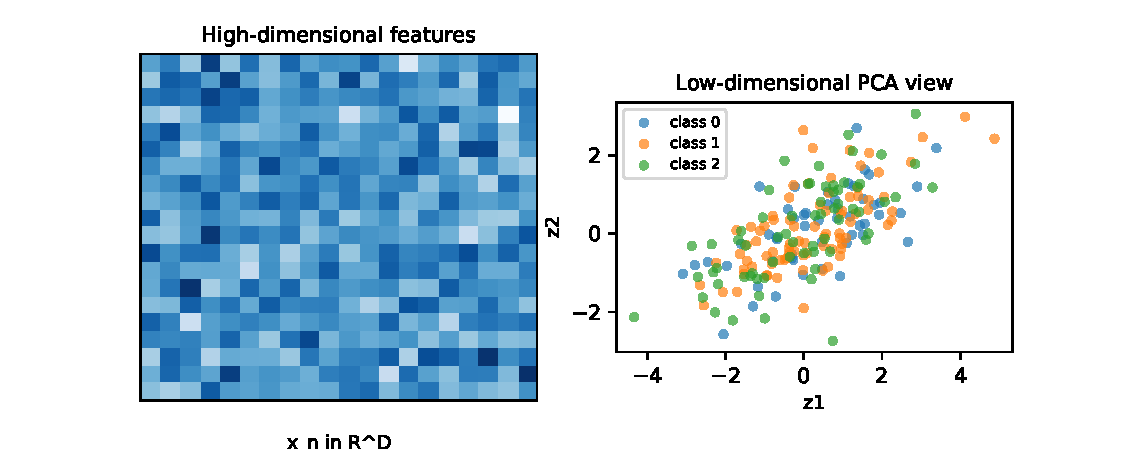
\includegraphics[width=0.7\textwidth]{pca_highdim2d_overview}
\end{figure}

\end{frame}


\section{Problem Setup}

\begin{frame}{Data and Linear Projection}

\textbf{Data matrix and centering}
\begin{itemize}
  \item We observe $N$ data points $\x_1, \dots, \x_N \in \mR^D$.
  \item We assume the data have been centered:
  \[
    \frac{1}{N}\sum_{n=1}^N \x_n = \zero.
  \]
  \item Centering simplifies the analysis and makes the origin a natural reference point.
\end{itemize}

\textbf{Linear projection onto one direction}
\begin{itemize}
  \item We first look for \emph{one} direction $\mathbf{u}_1 \in \mR^D$ onto which we project the data.
  \item For each data point $\x_n$, the scalar projection is
  \[
    z_{n1} = \mathbf{u}_1^{\top} \x_n.
  \]
  \item We constrain $\mathbf{u}_1$ to have unit length, $\|\mathbf{u}_1\|^2 = \mathbf{u}_1^{\top}\mathbf{u}_1 = 1$, so that the scale of the projection is well-defined.
\end{itemize}

\end{frame}


\begin{frame}{Sample Covariance and Projected Variance}

\textbf{Sample covariance matrix}
\begin{itemize}
  \item The (empirical) covariance matrix of the centered data is
  \[
    \mathbf{S} \defeq \frac{1}{N}\sum_{n=1}^N \x_n \x_n^{\top} \in \mR^{D \times D}.
  \]
  \item $\mathbf{S}$ captures how each pair of coordinates varies together.
\end{itemize}

\textbf{Variance along a direction}
\begin{itemize}
  \item The sample mean of the projections is zero:
  \[
    \frac{1}{N}\sum_{n=1}^N z_{n1}
    = \frac{1}{N}\sum_{n=1}^N \mathbf{u}_1^{\top}\x_n
    = \mathbf{u}_1^{\top}\bigg(\frac{1}{N}\sum_{n=1}^N \x_n\bigg)
    = 0.
  \]
  \item The sample variance of the projected data is
  \[
    \frac{1}{N}\sum_{n=1}^N z_{n1}^2
    = \frac{1}{N}\sum_{n=1}^N \big(\mathbf{u}_1^{\top}\x_n\big)^2
    = \mathbf{u}_1^{\top}\mathbf{S}\,\mathbf{u}_1.
  \]
  \item Thus, the variance along direction $\mathbf{u}_1$ can be written compactly as a quadratic form in $\mathbf{u}_1$.
\end{itemize}

\end{frame}


\begin{frame}{2D Toy Example of PCA}

\begin{figure}
  \centering
  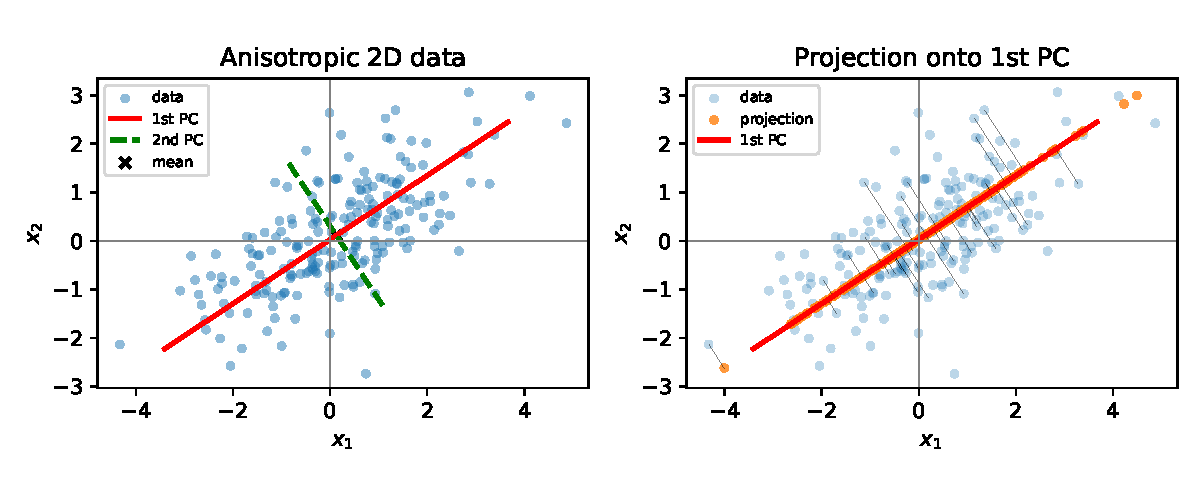
\includegraphics[width=0.8\textwidth]{pca_2d_example}
\end{figure}

\textbf{Interpretation}
\begin{itemize}
  \item \textbf{Left panel:} Anisotropic 2D data cloud together with the first (red) and second (green) principal axes and the sample mean (black cross).
  \item \textbf{Right panel:} The same data points, together with their orthogonal projections onto the first principal component (red line).
  \item Points are moved along short perpendicular segments to the red line; the coordinates on this line are exactly the one-dimensional PCA representation.
\end{itemize}

\end{frame}


\section{Maximum-Variance Formulation}

\begin{frame}{Optimization Problem for the First Component}

\textbf{Principle}
\begin{itemize}
  \item PCA chooses directions that \emph{maximize the variance} of the projected data.
  \item The first principal component $\mathbf{u}_1$ is the unit vector along which the projected data have the largest variance.
\end{itemize}

\textbf{Constrained optimization problem}
\begin{itemize}
  \item Using the expression for the variance, we want to solve
  \[
    \max_{\mathbf{u}_1} \;\; \mathbf{u}_1^{\top}\mathbf{S}\,\mathbf{u}_1
    \quad \text{subject to} \quad
    \mathbf{u}_1^{\top}\mathbf{u}_1 = 1.
  \]
  \item This is a quadratic objective with a quadratic (sphere) constraint.
  \item We can solve it using the method of Lagrange multipliers.
\end{itemize}

\end{frame}


\begin{frame}{Lagrangian and Eigenvalue Equation}

\textbf{Lagrangian}
\begin{itemize}
  \item Introduce a Lagrange multiplier $\lambda_1$ and define
  \[
    \cL(\mathbf{u}_1, \lambda_1)
    = \mathbf{u}_1^{\top}\mathbf{S}\,\mathbf{u}_1
      - \lambda_1(\mathbf{u}_1^{\top}\mathbf{u}_1 - 1).
  \]
\end{itemize}

\textbf{Stationary condition}
\begin{itemize}
  \item Taking the derivative with respect to $\mathbf{u}_1$ and setting it to zero gives
  \[
    \frac{\partial \cL}{\partial \mathbf{u}_1}
    = 2\mathbf{S}\,\mathbf{u}_1 - 2\lambda_1 \mathbf{u}_1
    = \zero.
  \]
  \item Hence, any stationary point satisfies
  \[
    \mathbf{S}\,\mathbf{u}_1 = \lambda_1 \mathbf{u}_1,
  \]
  which is the \emph{eigenvalue equation} for the covariance matrix $\mathbf{S}$.
\end{itemize}

\textbf{Choosing the largest eigenvalue}
\begin{itemize}
  \item One can show that the objective value at a stationary point is equal to the corresponding eigenvalue $\lambda_1$.
  \item Therefore, the maximum variance is obtained by choosing $\mathbf{u}_1$ to be the eigenvector of $\mathbf{S}$ associated with its largest eigenvalue.
\end{itemize}

\end{frame}


\begin{frame}{Subsequent Principal Components}

\textbf{Adding a second component}
\begin{itemize}
  \item After finding $\mathbf{u}_1$, we look for a second direction $\mathbf{u}_2$.
  \item We again maximize the variance of the projection
  \[
    z_{n2} = \mathbf{u}_2^{\top}\x_n,
  \]
  subject to $\|\mathbf{u}_2\|^2 = 1$.
  \item In addition, we require $\mathbf{u}_2$ to be orthogonal to $\mathbf{u}_1$:
  \[
    \mathbf{u}_1^{\top}\mathbf{u}_2 = 0.
  \]
\end{itemize}

\textbf{Result}
\begin{itemize}
  \item Solving this constrained problem again leads to an eigenvalue equation for $\mathbf{S}$.
  \item The optimal $\mathbf{u}_2$ is the eigenvector corresponding to the second largest eigenvalue of $\mathbf{S}$.
  \item Repeating this reasoning, we obtain a sequence of orthonormal eigenvectors
  \[
    \mathbf{u}_1, \mathbf{u}_2, \dots, \mathbf{u}_M,
  \]
  which form the first $M$ principal components.
\end{itemize}

\begin{figure}
  \centering
  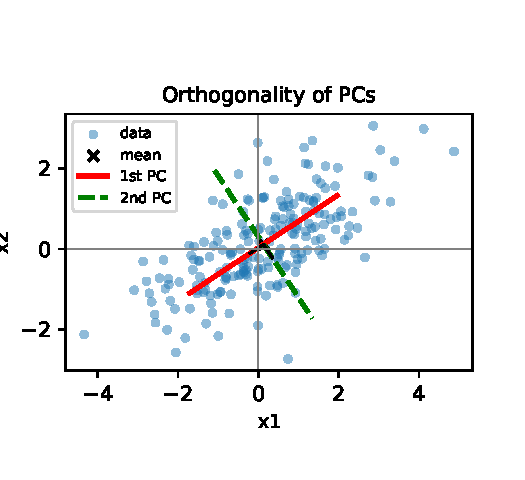
\includegraphics[width=0.55\textwidth]{pca_orthogonality}
\end{figure}

\end{frame}


\begin{frame}{Low-Dimensional Representation and Geometry}

\textbf{Low-dimensional coordinates}
\begin{itemize}
  \item Collect the first $M$ principal components into a matrix
  \[
    \U_M = [\mathbf{u}_1, \dots, \mathbf{u}_M] \in \mR^{D \times M}.
  \]
  \item The $M$-dimensional representation of $\x_n$ is
  \[
    \mathbf{z}_n = \U_M^{\top}\x_n \in \mR^M.
  \]
  \item These coordinates keep as much variance of the original data as possible among all linear $M$-dimensional projections.
\end{itemize}

\textbf{Geometric interpretation}
\begin{itemize}
  \item If the data cloud is roughly ellipsoidal, the eigenvectors of $\mathbf{S}$ give the principal axes of this ellipsoid.
  \item PCA aligns the coordinate system with these axes so that most of the spread lies in the first few coordinates.
  \item This is why PCA is often used for visualization (e.g., $M=2$) and as a preprocessing step for other learning algorithms.
\end{itemize}

\begin{figure}
  \centering
  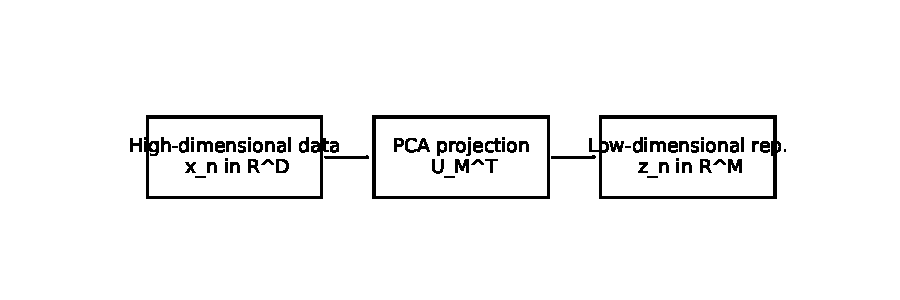
\includegraphics[width=0.65\textwidth]{pca_pipeline}
\end{figure}

\end{frame}


\begin{frame}{Summary of Section 12.1.1}

\begin{itemize}
  \item[(i)] Start from centered data $\x_1,\dots,\x_N \in \mR^D$ and compute the sample covariance matrix
  \[
    \mathbf{S} = \frac{1}{N}\sum_{n=1}^N \x_n \x_n^{\top}.
  \]
  \item[(ii)] The variance of the projection along a unit vector $\mathbf{u}$ is $\mathbf{u}^{\top}\mathbf{S}\,\mathbf{u}$.
  \item[(iii)] Maximizing this variance under the unit-norm constraint leads, via Lagrange multipliers, to the eigenvalue equation
  \[
    \mathbf{S}\,\mathbf{u} = \lambda \mathbf{u}.
  \]
  \item[(iv)] The principal components are the eigenvectors of $\mathbf{S}$, ordered by decreasing eigenvalues; they define directions of maximal variance in the data.
  \item[(v)] Projecting onto the first $M$ principal components yields an $M$-dimensional representation that preserves as much variance as possible among all linear projections.
\end{itemize}

\end{frame}

\begin{frame}[allowframebreaks]{References}
\bibliographystyle{apacite}
\nocite{bishop2006prml}
\bibliography{ref}
\end{frame}

\end{document}
